\documentclass[12pt]{article}


\usepackage[utf8]{inputenc}
\usepackage[a4paper,top=3cm,bottom=2cm,left=3cm,right=3cm,marginparwidth=1.75cm]{geometry}
\usepackage[nodayofweek]{datetime}
\usepackage{tabularx}
\usepackage[small]{titlesec}
\usepackage{graphicx}
\usepackage{tabularx}
\usepackage{amsmath}
\usepackage{upgreek}
\usepackage{fancyvrb}
\newcolumntype{L}[1]{>{\raggedright\arraybackslash}p{#1}}
\newcolumntype{C}[1]{>{\centering\arraybackslash}p{#1}}
\newcolumntype{R}[1]{>{\raggedleft\arraybackslash}p{#1}}

\begin{document}
    

\begin{titlepage}
    \begin{center}
        \huge{\bfseries  Tribhuvan University}\\
        \Large{Institute of Engineering}\\
        \huge{ \bfseries  Pulchowk Campus}\\[3.2cm]


        \textsc{\Large Digital Signal Analysis and Processing}\\[-0.5cm]
        \line(1,0){400}\\
        \huge{\bfseries Lab 3}\\
        \huge{Convolution}
        \line(1,0){400}\\


        \textsc{\Large Submitted by:}\\
        \Large Bishal Katuwal\\ \large 075BCT028\\    [0.85cm]

        \textsc{\Large Submitted to:}\\\
        \large Department of Electronics and Computer Engineering\\Pulchowk Campus\\    [0.85cm]
        
        \textsc{\Large Submitted on:}\\
        \today
        
    \end{center}
\end{titlepage}
\pagebreak
% ===============================================================
\paragraph{Title\\}
Convolution
% ===================================================
\paragraph{Background Theory}
\subparagraph{Definition\\}
In mathematics, convolution is a mathematical operation on two functions (f and g) that produces a third function (f*g) that expresses how the shape of one is modified by the other. 
The term convolution refers to both the result function and to the process of computing it. 
It is defined as the integral of the product of the two functions after one is reversed and shifted. 
The integral is evaluated for all values of shift, producing the convolution function.
\begin{equation}
	(f * g)(t) := \int_{-\infty}^\infty f(\uptau)g(\uptau-t)\mathrm{d}\uptau
\end{equation}
Similarly the discrete convolution is given as:
\begin{equation}
	(f * g)[n] := \sum_{-\infty}^\infty f[m]g[n-m] 
\end{equation}
\subparagraph{Convolution in MATLAB\\}
\begin{verbatim}
w = conv(u,v)
\end{verbatim}
 where w is the convolution of u and v.
\begin{verbatim}
Convolution is commutative
\end{verbatim}
% ===============================================
\pagebreak
\paragraph{Activities\\}
\begin{enumerate}
    \item {Find the convolution of\\
        \begin{enumerate}
            \item $x[n] = [1.2, 2.3, 4.6, -5, -11.6]$ and $h[n] = [2,3,1.7,2.9]$
                \begin{Verbatim}[frame=single]
x = [1.2, 2.3, 4.6, -5, -11.6]
h = [2,3,1.7,2.9]
y = conv(x,h)

subplot( 3, 1, 1);
stem(x);
title('x')

subplot( 3, 1, 2);
stem(h);
title('h')

subplot( 3, 1, 3);
stem(y);
title('y = x*h')
                \end{Verbatim}
             \begin{figure}[h!]
                \centering
                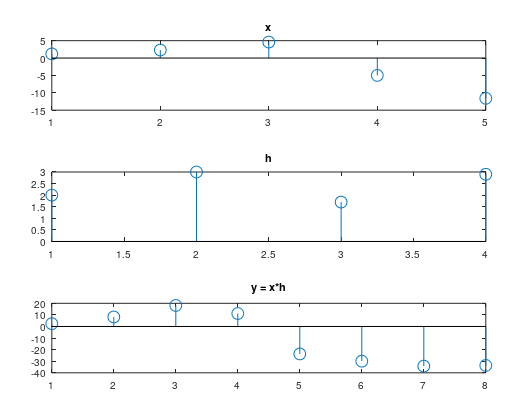
\includegraphics{labss/Convolution1a.PNG}
                \caption{$x[n] = [1.2, 2.3, 4.6, -5, -11.6]$ and $h[n] = [2,3,1.7,2.9]$}
             \end{figure}   
            \pagebreak
             \item $x[n] = 1$ for $0	\leq n \leq 5$ and $h[n] = 0.7$ for $-1	\leq h	\leq 3$
            \begin{Verbatim}[frame=single]
1;
function x = pieceWise(t,l,u)
  x = zeros (size (t));
  ind = t >= l & t <= u;
  x(ind) = 1;
endfunction

tx1 = 0;tx2=5
tx = tx1:tx2
x = pieceWise (tx,tx1,tx2);
subplot( 3, 1, 1);
stem (tx,x)

th1 = -1; th2=3
th = th1:th2
h = 0.7 * pieceWise (th,th1,th2);
subplot( 3, 1, 2);
stem (th,h)

ty = ((tx1+th1):1:(tx2+th2))
y = conv(x,h)
subplot( 3, 1, 3);
stem (ty,y)
            \end{Verbatim}
            \begin{figure}[h!]
                \centering
                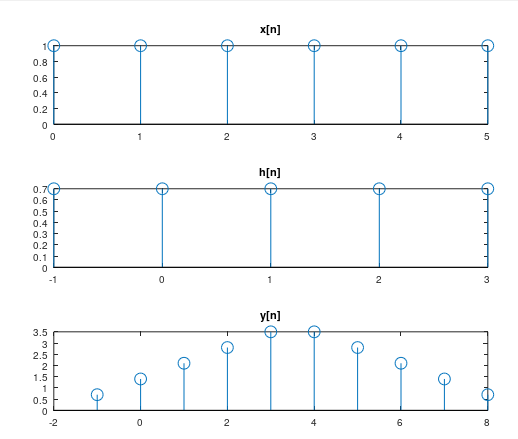
\includegraphics{labss/Convolution1b.PNG}
                \caption{$x[n] = 1$ for $0	\leq n \leq 5$ and $h[n] = 0.7$ for $-1	\leq h	\leq 3$}
             \end{figure}   
             \pagebreak
            \item $x[n] = a^n u[n]$ where $0 \leq a \leq 1$ and $h[n] = u[n]$
            \begin{Verbatim}[frame=single]
n = 0:1:10
a = 0.5

x = [a.^(0:10)];
subplot( 3, 1, 1);
stem (n,x)
title('x[n]')

h = [1.^(0:10)];
subplot( 3, 1, 2);
stem (n,h)
title('h[n]')

y = conv(x,h);
subplot( 3, 1, 3);
stem (y)
title('y[n]')
            \end{Verbatim}
            \begin{figure}[h!]
                \centering
                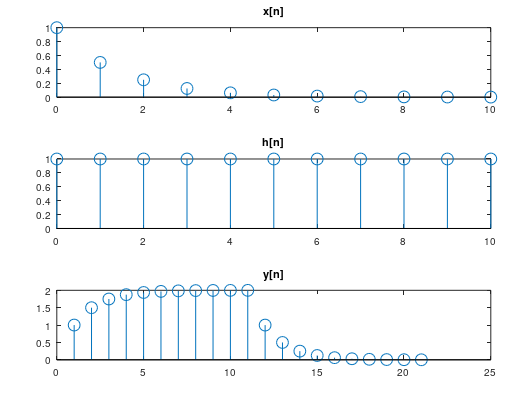
\includegraphics{labss/Convolution1c.PNG}
                \caption{ $x[n] = a^n u[n]$ where $0 \leq a \leq 1$ and $h[n] = u[n]$}
             \end{figure}   
             \pagebreak
            \item $x(t) = u(t) - u(t-3)$ and $h(t) = u(t)$
             \begin{Verbatim}[frame=single]
n = 0 : 1 : 10

x = (n >= 0) - (n >= 3)
subplot( 3, 1, 1);
plot (n,x)
title('x(t)')

h = (n >= 0)
subplot( 3, 1, 2);
plot (n,h)
title('h(t)')

y = conv(x,h);
subplot( 3, 1, 3);
plot (y)
title('y(t)')

             \end{Verbatim}
             \begin{figure}[h!]
                \centering
                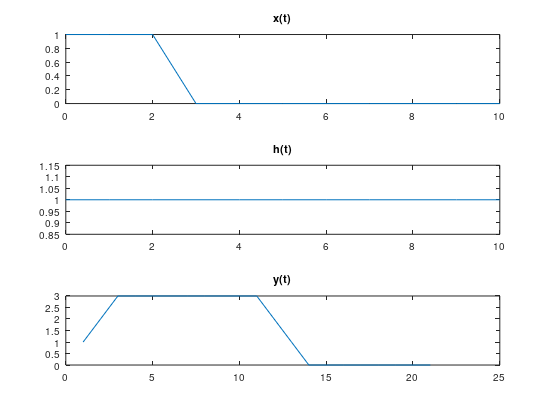
\includegraphics{labss/Convolution1d.PNG}
                \caption{ $x(t) = u(t) - u(t-3)$ and $h(t) = u(t)$}
             \end{figure}   
             \pagebreak
        \end{enumerate}
    }
    \item Find convolution of\\ 
    $x[n] = [1.2, 2.3, 4.6, -5, -11.6]$ and $h[n] = [2,3,1.7,2.9]$ \\
    using your own convolution function.
    \begin{Verbatim}[frame =single]
x = [1.2, 2.3, 4.6, -5, -11.6]
subplot( 4, 1, 1);
stem(x);
title('x')

h = [2,3,1.7,2.9]
subplot( 4, 1, 2);
stem(h);
title('h')

%y=conv(x,h)
subplot( 4, 1, 3);
stem(conv(x,h));
title('Inbuild convolution')

len_h = length(h);
len_x = length(x);

H=[h,zeros(1,len_x)];
X=[x,zeros(1,len_h)];

for i=1:len_h+len_x-1
    Y(i)=0;
    for j=1:len_x
        if(i-j+1>0)
            Y(i)=Y(i)+X(j)*H(i-j+1);
        else
        end
    end
end

subplot( 4, 1, 4);
stem(Y);
title('Manual conv')
    \end{Verbatim}
    \begin{figure}[h!]
        \centering
        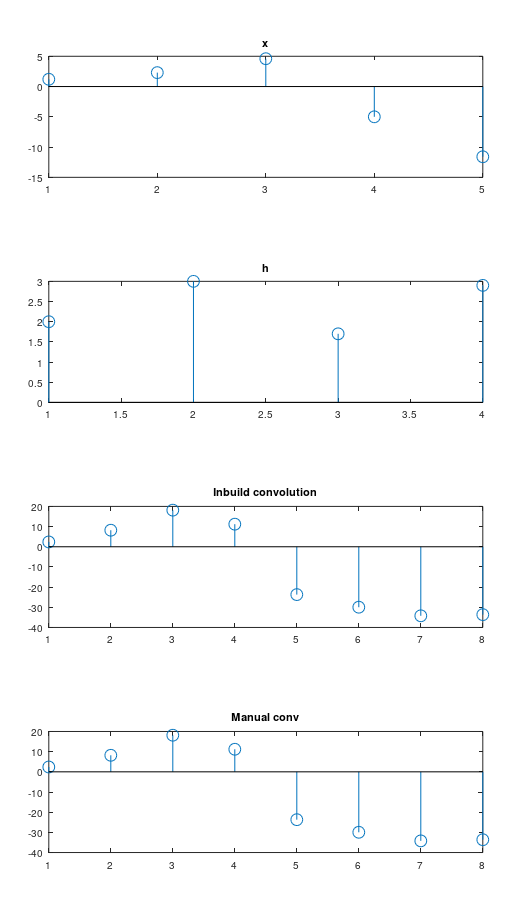
\includegraphics[scale=0.8]{labss/Convolution2.PNG}
        \caption{ x[n] = [1.2, 2.3, 4.6, -5, -11.6] and h[n] = [2,3,1.7,2.9]}
     \end{figure}   
     \pagebreak
\end{enumerate}

% ===============================================
\pagebreak
\paragraph{Conclusion\\}
In this way "Lab 3 : Convolution" was completed by performing convolution for both discrete and continuous signals.
Also, a convolution function of our own was created for discrete signals.

\end{document}